% !TeX spellcheck = en_US
\documentclass[12pt]{article}
\usepackage[unicode=true]{hyperref}
\usepackage[utf8x]{inputenc}
\usepackage{amsmath,amsthm,amsfonts,eucal}
\usepackage{graphicx}
\usepackage{placeins}


\title{Applications of the Fresnel Integrals}
\author{Jack Jones}
\date{March 17\th, 2019}


\newcommand\defbb[2]{\def#1{{\mathbb{#2}}}}
\newcommand\defbf[2]{\def#1{{\mathbf{#2}}}}
\newcommand\defcal[2]{\def#1{{\mathcal{#2}}}} % capital letters only
\newcommand\defrm[2]{\def#1{{\mathrm{#2}}}}
\newcommand\defsf[2]{\def#1{{\mathsf{#2}}}}
\newcommand\defvec[2]{\def#1{{\vec{#2}}}}
\def\vec{\mathbf}
\renewcommand\th[1][th]{$^{\text{#1}}$}
\newtheorem*{thm}{Theorem}

\let\C=\relax
\DeclareMathOperator\C{C} % \C(x) := \int_0^x cos(\pi/2*t^2) \d{t}
\defbb\CC{C} % complex numbers
\defrm\ud{d}
\def\d#1{{\,\ud#1\,}}
\newcommand\udfrac[2]{\ensuremath{\frac{\ud#1}{\ud #2}}}
\defrm\e{e}  % Euler's number
\DeclareMathOperator\erf{erf} % error function
\defsf\si{i} % \sqrt{-1}
\defbb\R{R}
\let\para=\S
\let\S=\relax
\DeclareMathOperator\S{S} % \S(x) := \int_0^x sin(\pi/2*t^2) \d{t}


\begin{document}\def§{{\ensuremath{\para}}}
\maketitle
\begin{abstract}

The Euler spiral, that is defined by the linear relationship between curvature and arc length, is a beautiful and elegant plane curve. Its underlying mathematical equation is most
commonly known as the Fresnel integrals. However, the Fresnel integrals and Euler spiral are  two views of one and the same thing. In this paper, we focus on the Fresnel integrals and study its properties and useful applications. In optics, the illumination intensity at a point behind a straight edge is computed from the distance between two points on the Euler spiral. The Euler spiral also provides optimal curvature for train tracks between a straight run and an upcoming bend.

\end{abstract}
\clearpage


\section{Introduction}
An Euler spiral is a curve whose curvature changes linearly with its arc length. Taking the example of peeling an orange with a kitchen knife, one can either cut the skin along meridians, or cut it along a spiral as the left-hand image in Figure~\ref{f:orangePeel} shows. The red lines marked on the orange refer to the route one can follow to peel the orange. Later, if we unfold the spiral strip and flatten it on a table, we will see a long curve which is curved differently at different positions. Imagine that we will now cut the peel with progressively thinner strip widths, what we will obtain in the end is a long beautiful curve known as Euler spiral, as the right-hand image in Figure~\ref{f:orangePeel} shows. According to Alfred Gray, Euler spiral is “one of the most elegant of all plane curves.” \cite{ASG17}


\begin{figure}[h!]
	\centering
	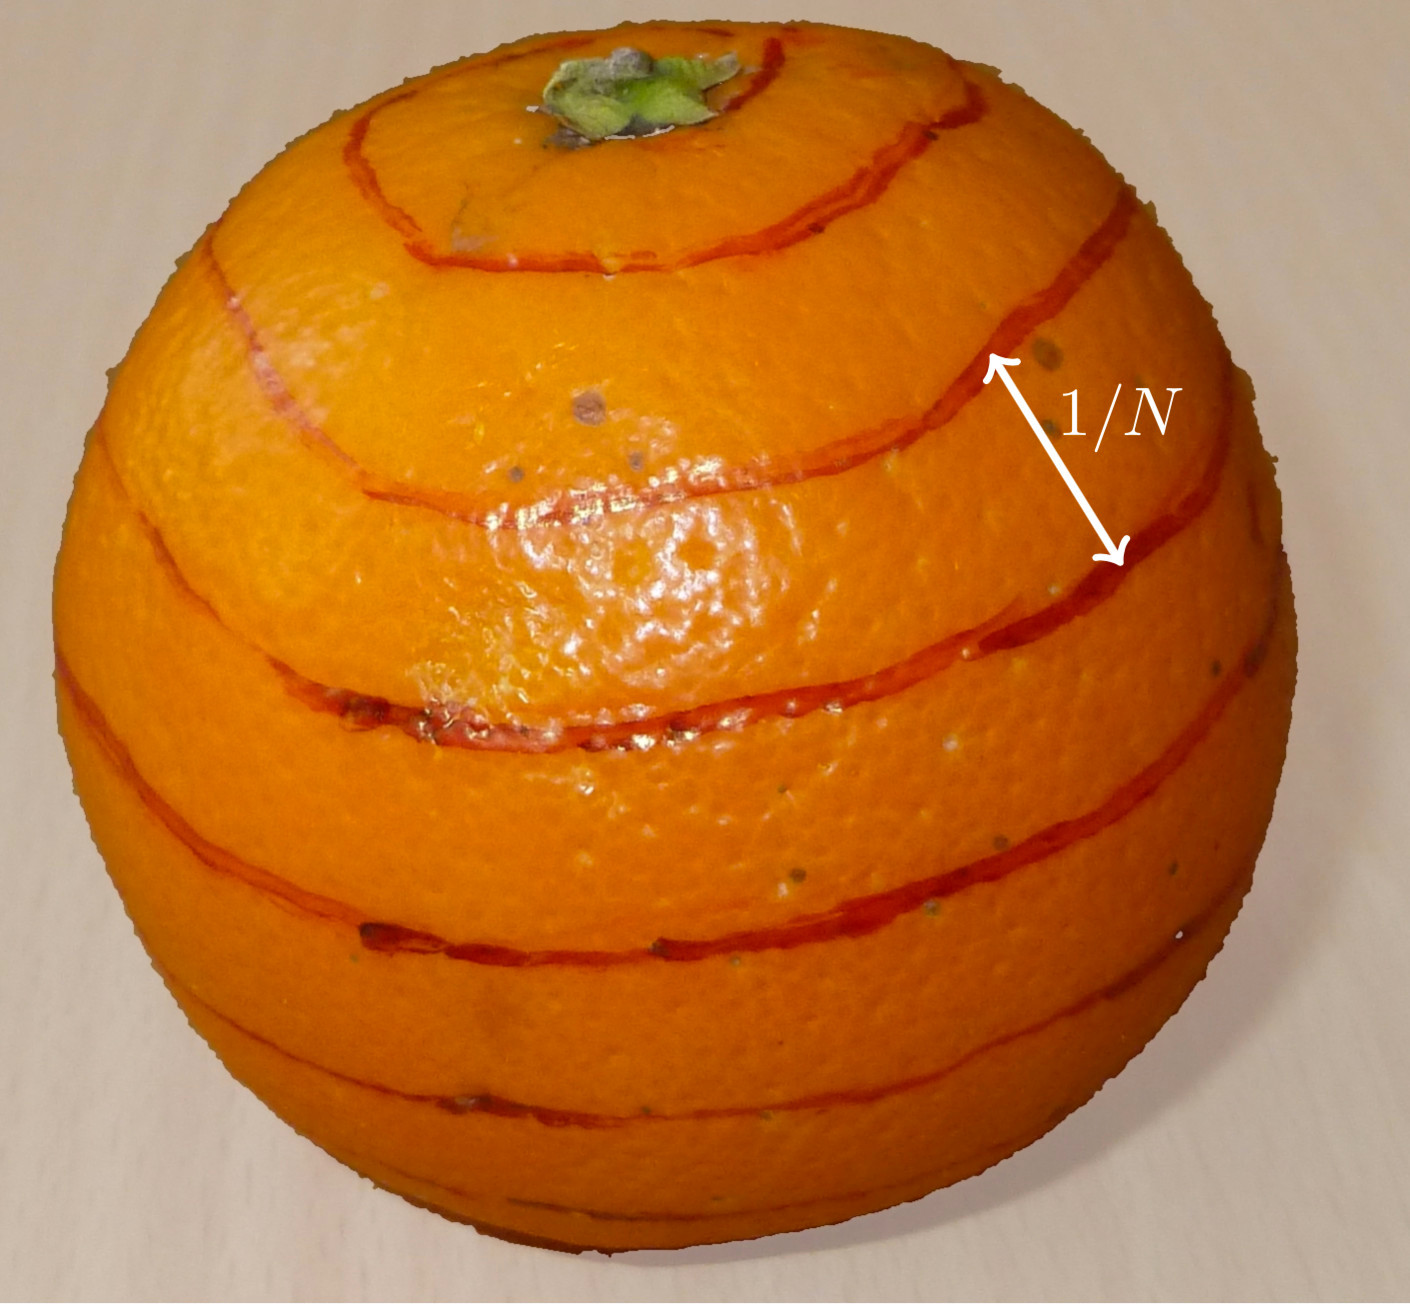
\includegraphics[height=5cm]{orange.jpg} \hfill
	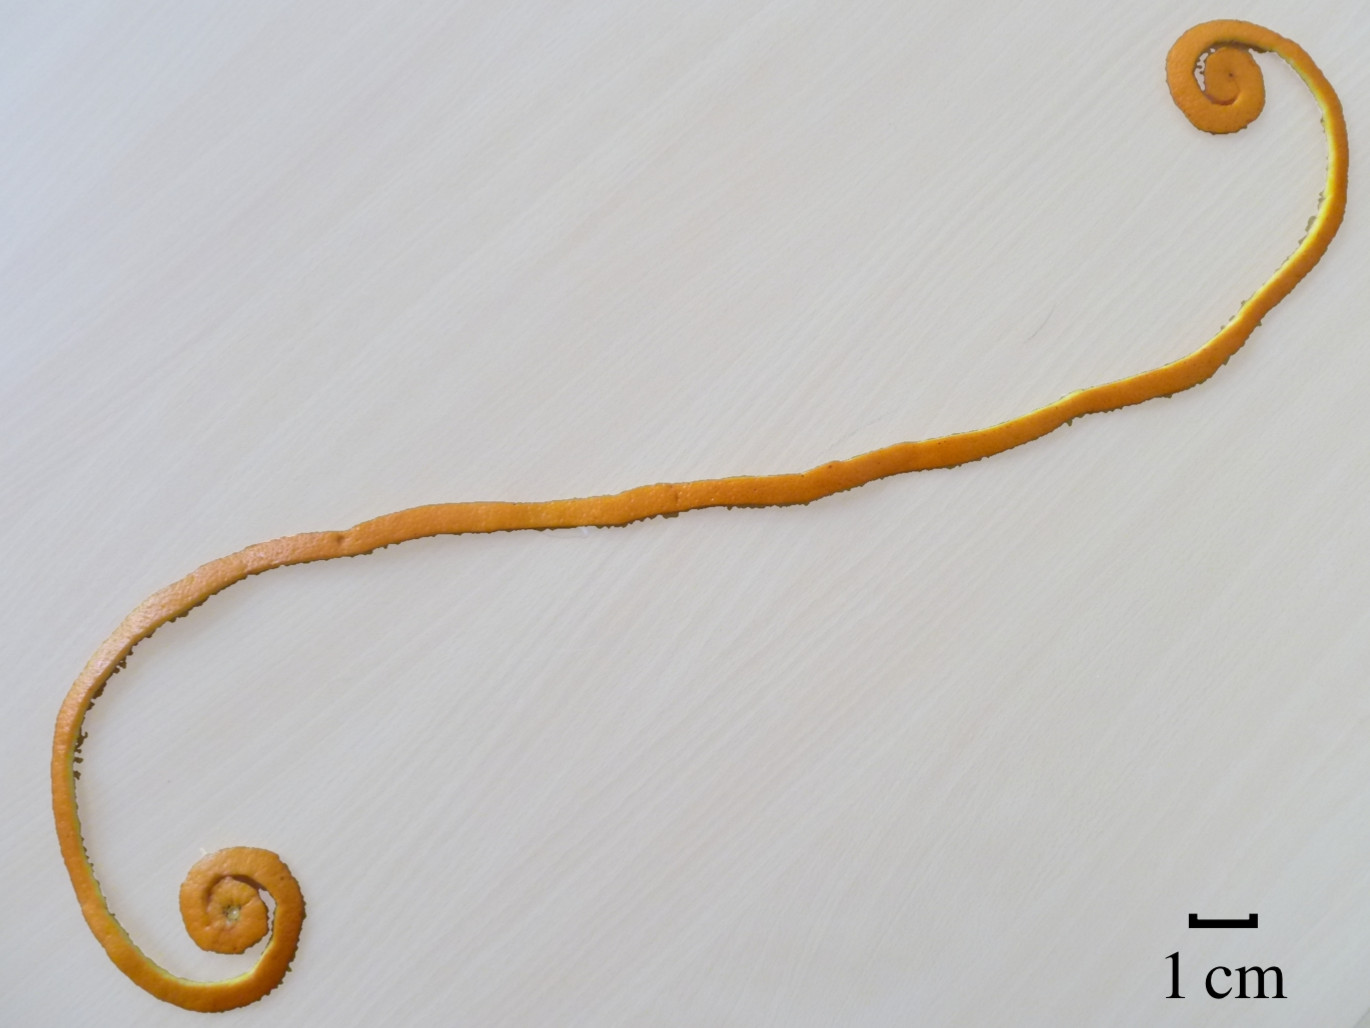
\includegraphics[height=5cm]{orangePeel.jpg}
	\label{f:orangePeel}
	\caption{Left: Peeling an orange in a spiral of height $1/N$.
		Right: The flattened orange peel that resembles an Euler spiral.  Photos taken from \cite{BH12}.
	}
\end{figure}

For a mathematician, an interesting question is whether there are any equations that can describe the corresponding shape of an Euler spiral. For this we consider the Fresnel integrals.  These are defined as integrals over some elementary functions which can however not be integrated in elementary functions.  These integrals occur naturally in the description of the optics of an illuminated straight edge (see Subsection~\ref{s:relation}).


\subsection{Definition of Euler Spiral}
The Euler Spiral is defined by the  linear relationship between curvature and arc length and was
first proposed as a problem of elasticity by James Bernoulli, then solved accurately by Leonhard Euler \cite{Lev08}.
The Euler spiral is a curve in the complex plane that has curvature proportional to the arc length.  Here the arc length $s(t)$ of a differentiable curve $(x(t),y(t))$ in the plane is defined by
\[  \left(\udfrac{s}{t}\right)^2 := \left(\udfrac{x}{t}\right)^2 +\left(\udfrac{y}{t}\right)^2.
\]  Note that the arc length is monotone increasing with the parameter $t$ of the curve.  For a nice curve, it is possible to rewrite the curve in the arc length, i.e.~$(x(s),y(s))$.

The curvature $\kappa$ of a smooth curve can be defined as 
\[  \kappa=\frac1R = x'y'' -x''y'
\] if we assume that the curve is parameterized in the arc length $s$ \cite{BH12}.  The meaning is that at a point $(x(s),y(s))$ we approximate the curve by a circle segment that touches in this point of at least second order.  Then $R$ is the radius of this touching circle and $\kappa$ its inverse.

According to \cite{BH12} the peel of the orange can be approximated as
\begin{equation}
  \kappa \sim s  \label{e:eulerSpiral}.
\end{equation}  This is the differential equation of the Euler curve.  The goal is to find all smooth curves $(x(s),y(s))$ whose curvature is in every point as described.

The question we want to answer is how to describe the solution of this differential equation explicitly.  Therefore we introduce the Fresnel integrals.


\subsection{Definition of the Fresnel Integrals}
The Fresnel sine and cosine integrals are represented by $\S(x)$ and $\C(x)$, which are two integral functions that originate by applying the analysis of Fresnel diffraction phenomena. The mathematical equations are as follows:

\begin{align}
  \S(x) &:= \int_0^x  \sin\left(\frac\pi2 t^2\right) \d{t}, \\
  \C(x) &:= \int_0^x \cos\left(\frac\pi2 t^2\right) \d{t},
\end{align}
where $x$ is a real number and $t$ is a real variable. When $x$ tends to infinity, $\S=\C=1/2$.

The difficulty is that these integrals cannot be computed with analytic means, i.e.~the functions are transcendental \cite[p.195ff]{AS}.  This is in contrast to, e.g.
$$ \int_0^x (\sin t)^2 \d{t} = \frac12\int_0^x \left(1-\cos(2t)\right)\d{t} = \frac12x -\frac14\sin(2x).
$$


\subsection{Mathematical history}
The Fresnel integral and the related Euler spiral were discovered multiple times during history.  One of the first occurrences is according to \cite{Lev08} by J. Bernoulli in 1694 where he defines a curve such that an ideal metal rod of this shape unwinds to a straight line when placed under load at the ends.  In 1744, Euler is able to describe the curve by a differential equation that also allows him to reformulate it as the Fresnel integral.  37 years later he is able to compute the limiting points ($t\to\pm\infty$) of the curve and integrals.  Fresnel discovers the curve in 1818 independently and successfully applies it to the diffraction on a slit \cite{Lev08}.  He is also able to compute a couple of values numerically.  In 1874 Cornu plotted the curve accurately and proposes it as a graphical means for computing diffraction problems.

In the following sections, we will first describe the important properties of the Fresnel integrals followed by some important applications of it.

\section{Properties of the Fresnel Integrals}
\subsection{Basic properties}
The Fresnel integrals are odd, i.e.
\begin{align*}
	\S(-x) &= \S(x), & \C(-x) &= \C(x).
\end{align*}
\begin{proof}[Idea of proof]  The integrands $\sin(t^2)$ and $\cos(t^2)$ are even in $t$ and an anti-derivative $F(x)$ of an even function is odd if in addition $F(0)=0$.  The latter follows, because both integrals start at $t=0$.
\end{proof}

Their limits are
\[  \lim_{x\to\infty} \S(x) = 0.5,\qquad  \lim_{x\to\infty} \C(x) = 0.5.
\]

Since the integrals cannot be computed by elementary analytic means, an alternative is to compute them with a power series.  Therefore we present the Taylor expansion as
\begin{align*}
  \S(x) &= \sqrt{\frac\pi2}\sum_{n\ge0} (-1)^nx^{4n+3}\frac{(\pi/2)^{2n+1}}{(2n+1)!(4n+3)}, \\
  \C(x) &= \sqrt{\frac\pi2}\sum_{n\ge0} (-1)^nx^{4n+1}\frac{(\pi/2)^{2n}}{(2n)!(4n+1)}.
\end{align*}
\begin{proof}[Idea of proof]  Start from the well known Taylor expansion of $\sin t = \sum_{n\ge0}$ $(-1)^n t^{2n+1}/(2n+1)!$ and $\cos t = \sum_{n\ge0} (-1)^nt^{2n}/(2n)!$, substitute $t\mapsto \tfrac\pi2 t^2$ and take the antiderivative for each summand.  The resulting series are $\S(t)$ and $\C(t)$, because the integral of an absolutely converging power series equals the absolutely converging power series of the integrals of the summands.
\end{proof}

\begin{figure}[h!]
	\centering
	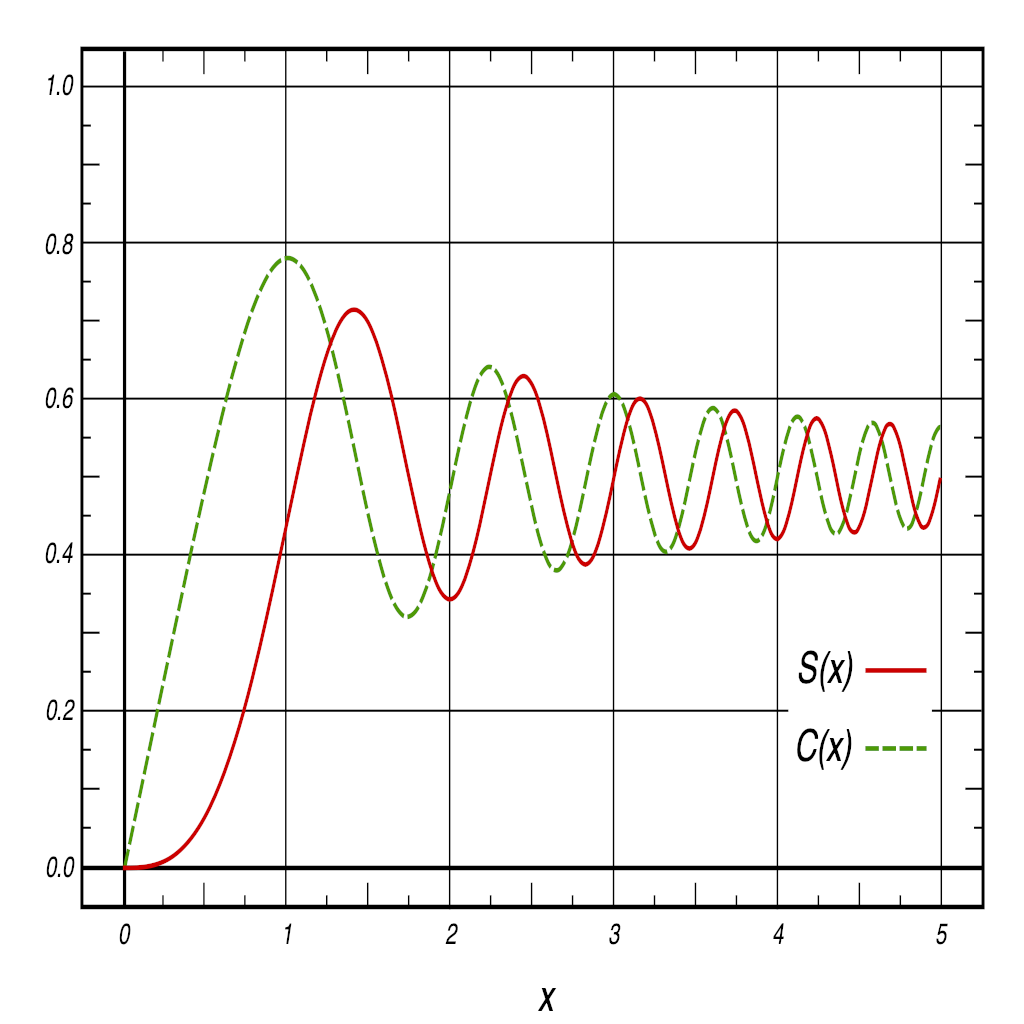
\includegraphics[width=0.4\textwidth]{Fresnel-Integrals-(Normalised).png}
	\caption{Fresnel integrals \cite{wiki}.}
\end{figure}

\FloatBarrier
\subsection{Relation to the Euler spiral}\label{s:relation}
\begin{thm}  The curve $(x,y)=(\C(t),\S(t))$ is an Euler spiral.
\end{thm}
\begin{proof}  Let us start with showing that $t$ is the parameter of the arc length.  Consider therefore the derivatives
\begin{align*}
  \C'(t) &= \cos\left(\frac\pi2 t^2\right), &  
  \S'(t) &= \sin\left(\frac\pi2 t^2\right), \\
  \C''(t) &= -\frac\pi2\sin\left(\frac\pi2 t^2\right)\cdot 2t, &
  \S''(t) &= \frac\pi2\cos\left(\frac\pi2 t^2\right)\cdot 2t.
\intertext{Then}
  \left(\udfrac{s}{t}\right)^2 &= (C'(t))^2+(S'(t))^2 = 1
\end{align*}
i.e.~$t$ is the arc length $s$ of the curve.

Let us now consider the curvature
\begin{align*}
  \kappa &= x'y''-x''y' = C'(t)S''(t)-C''(t)S'(t) = \frac{\pi}{2}2t \sim t
\end{align*}
\end{proof}

\begin{figure}[h!]
	\centering
	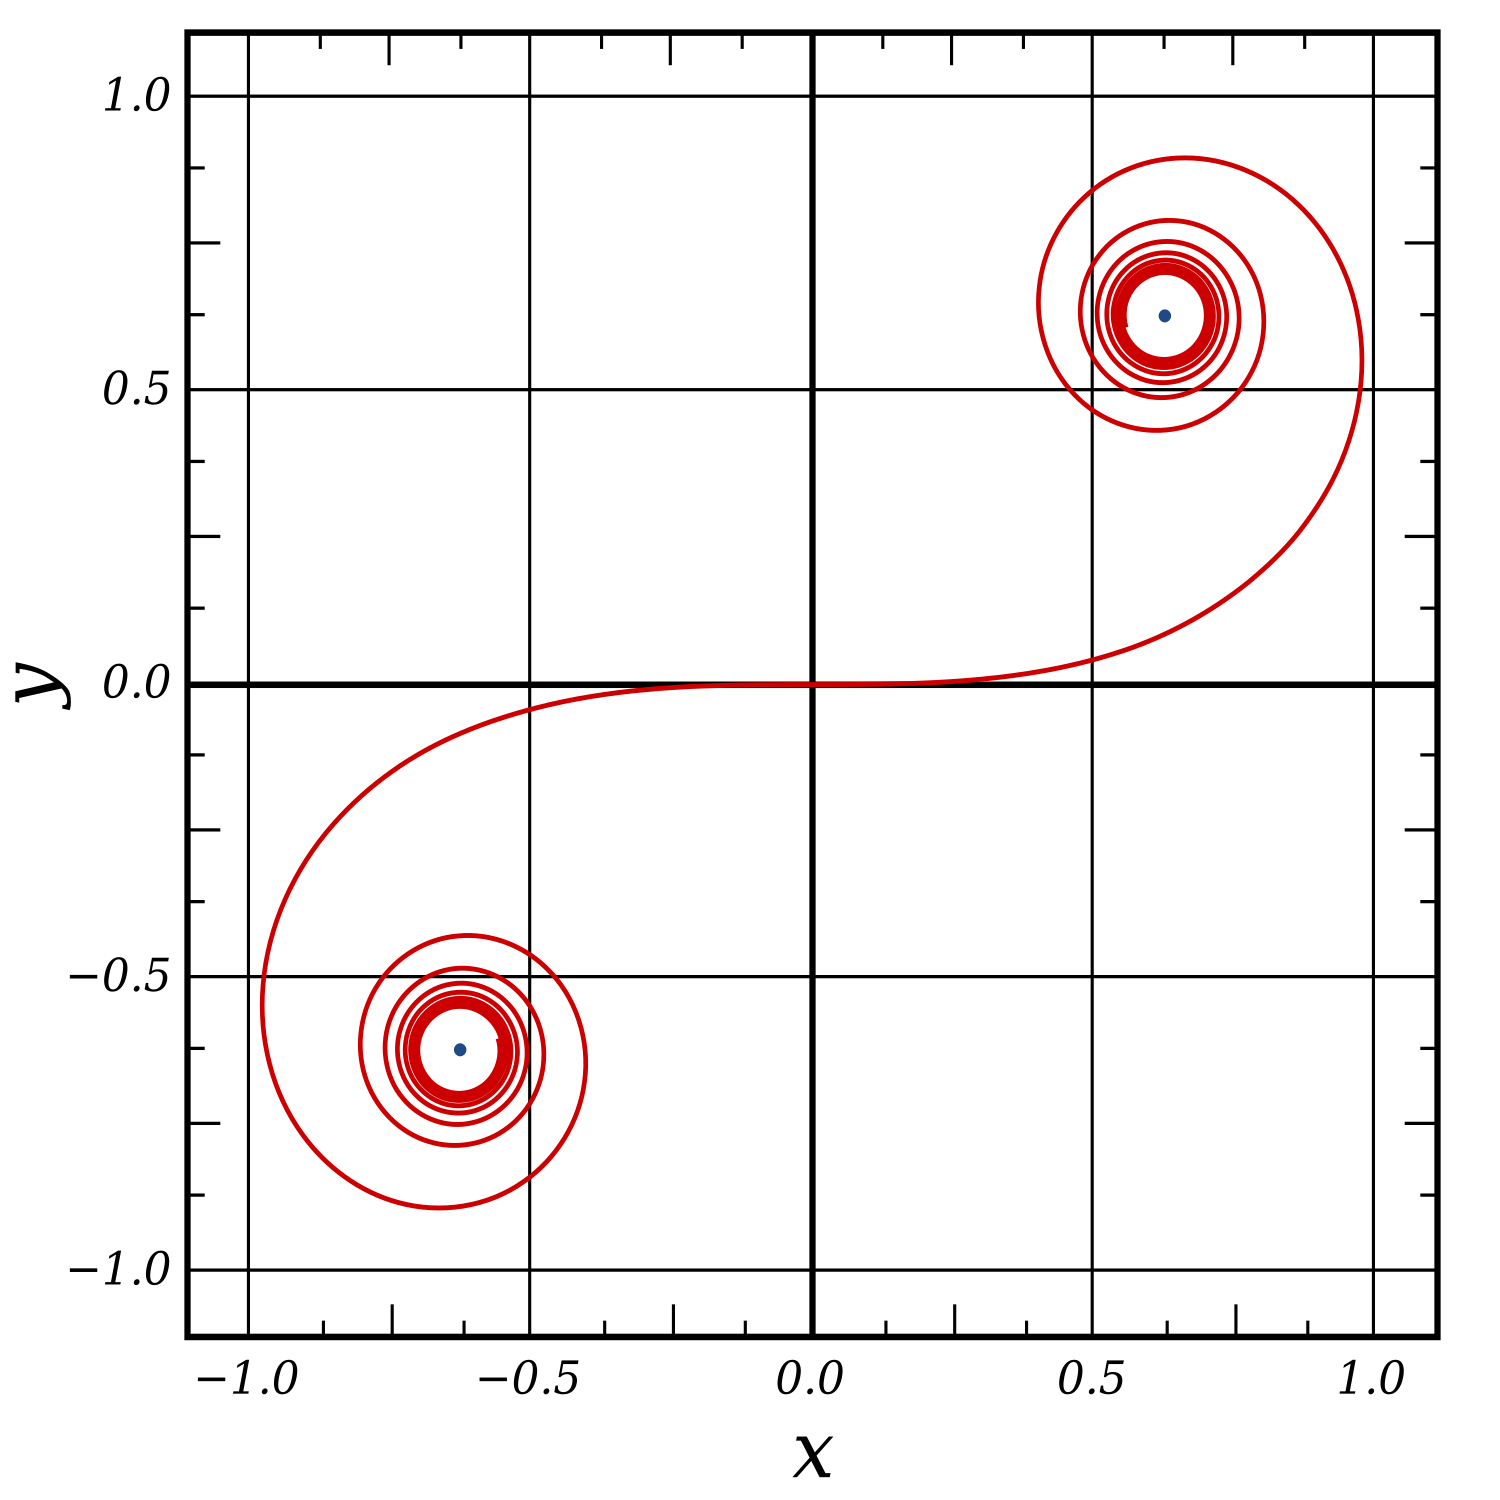
\includegraphics[width=0.5\textwidth]{eulerSpiral.png}
	\label{f:eulerSpiral}
	\caption{Euler spiral $(x,y)=(\C(t),\S(t))$ \cite{wiki}.}
\end{figure}


\subsection{Other expressions}
The Fresnel integrals are closely related to the error function which is defined as follows
$$  \erf(x) := \int_{-x}^x \exp(-t^2) \d{t}.
$$
Also this function is analytic and can therefore be expanded to the whole complex plane.  Here the integral for fixed endpoints is independent of the path.

Now for the complex definition of exponential function
\begin{align*}  \exp(x+\si y) &:= (\cos y +\si\sin y)\e^x
\intertext{we obtain}
  \C(z)+\si\S(z) &= \int_0^z \exp\left(\si\frac\pi2 t^2\right)\d{t} 
\intertext{Now we do a substitution in the complex plane as $t'=\sqrt{\si\frac\pi2}t$, i.e.~$\d{t'}=\frac{1+\si}{\sqrt{2}}\sqrt{\frac\pi2}\d{t}$ and obtain}
  &= \frac{1-\si}{\sqrt{2}}\sqrt{\frac2\pi}\int_0^{\frac{1+\si}{\sqrt{2}}\sqrt{\frac\pi2}z} \exp(t^{\prime2}) \d{t'} = \frac12\sqrt{\frac2\pi}\,\frac{1-\si}{\sqrt2} \erf\left(\frac{1+\si}{\sqrt2}\,\sqrt{\frac\pi2} z\right).
\end{align*}
Therefore we can say that the Fresnel integrals are the real and imaginary part of the complex error function.


\section{Applications of the Fresnel Integrals}
Fresnel Integrals and Euler spiral have applications in many fields of science. They occurred originally in the analysis of the diffraction of light. More recently, Euler spiral appears in the design of highways and railroad tracks, robot trajectory planning, and computer-aided design. In this section, we will describe two main applications of the Fresnel integrals in detail, namely the original Fresnel Diffraction and the railway construction. 


\subsection{Fresnel Diffraction}
\defbf\E{E}
\defbf\B{B}
\begin{figure}[h!]
	\centering
	\includegraphics[width=0.5\textwidth]{opticalSetting.png} \\
	% (2) \includegraphics[width=0.5\textwidth]{opticalParameters.png}
	\label{f:FresnelDiffraction}
	\caption{Fresnel diffraction after \cite[ch.~8.1]{Zim08}. Incoming parallel light waves from the left.  An aperture S' and an observation screen on the right in distance $D$.}
\end{figure}
According to \cite[ch.~7]{Zim08} the complexified electric field strength $\E$ at a point $P$ on the observation screen of a plane electromagnetic wave that went through an aperture $S'$ computes as
\[  \E(P) = \B\iint  \frac1\rho \exp\left(\si(k\rho-\omega t)\right) \d{S'}
\] where $\B$ determines the amplitude of the incoming wave,\\ $\rho=\sqrt{(x-x')^2+(y-y')^2+D^2}$ is the distance of the aperture point $S'$ from the observation point $P$.  $k=\omega/c$ is the wave number, $\omega>0$ the frequency of the incoming monochromatic wave and $c>0$ the speed of light.  In the Fresnel approximation we assume that $|x-x'|/D\ll 1$ and $|y-y'|/D\ll 1$, but will not assume that the aperture itself is small.  Therefore we expand in the lowest orders of $(x-x')/D$ and $(y-y')/D$ and obtain
\[  \E(P) \approx \B\frac{\exp\left(\si(kD-\omega t)\right)}{D} \iint \exp\left(\si(x'-x)^2k/2D +\si(y'-y)^2k/2D\right) \d{(x',y')}.
\]  If we combine the constant coefficient as $\E_0$ and assume a rectangular aperture of size $[x_0,x_1]\times[y_0,y_1]$, we obtain
\begin{align*}  \E(x,y) &\approx \E_0 \int_{u_0}^{u_1} \exp\left(\si\frac\pi2 u^2\right)\d{u} \int_{v_0}^{v_1} \exp\left(\si\frac\pi2 v^2\right) \d{v} \\
  &= \E_0 \left[\C(u_1)+\si\S(u_1)-\C(u_0)-\si\S(u_0)\right] \left[\C(v_1)+\si\S(v_1)-\C(v_0)-\si\S(v_0)\right]
\end{align*} where $u_k:=\sqrt{\frac2{D\lambda}}(x_k-x)$, $v_k:= \sqrt{\frac2{D\lambda}}(y_k-y)$ for $k=0,1$ \cite[Eqns.~(8.34a\&b)]{Zim08} and $\lambda=2\pi/k$ is the wave length.  The intensity near a vertical edge results as
\[  I(x):= |\E|^2 = \frac{I_0}{2} \left[\left(\frac12-\C(u_0)\right)^2+\left(\frac12-\S(u_0)\right)^2\right].
\] See also \cite[Eqn.~(8.38)]{Zim08}.  This formula is the distance along the Euler spiral between the right point at $t=\infty$ and the left point at $t=u_0$.


\FloatBarrier 
\subsection{Railway  Construction}

An object traveling on a circular path experiences a centripetal acceleration. The same happens when a train that travels on a straight path suddenly transitions to a tangential circular path. This sudden centripetal acceleration causes much discomfort for the driver as well as the passengers on the train. 

In order to provide a smooth riding experience, much effort has been made in the history of railway construction. According to \cite{Lev08}, Mr. Gravatt was the first one who designed a sine curve around the year of 1828. Later by 1842, William Froude proposed to use a curve approximating the elastic curve, for the purpose of making the change of curvature by degree. In the year of 1880, Charles Crandall gives priority for the ``true transition curve'' to Ellis Holbrook in the Railroad Gazette. However, Arthur Talbot was among the first to approach the problem mathematically as he describes the problem and his solution in the introduction to ``The Railway Transition Spiral'' \cite{Tal99}:

\begin{quotation}
	A transition curve, or easement curve, as it is sometimes called, is a curve of varying radius
	used to connect circular curves with tangents for the purpose of avoiding the shock and
	disagreeable lurch of trains, due to the instant change of direction and also to the sudden
	change from level to inclined track. The primary object of the transition curve, then, is to
	effect smooth riding when the train is entering or leaving a curve.
	
	The generally accepted requirement for a proper transition curve is that the degree-of-curve
	shall increase gradually and uniformly from the point of tangent until the degree of the main
	curve is reached, and that the super-elevation shall increase uniformly from zero at the
	tangent to the full amount at the connection with the main curve and yet have at any point
	the appropriate super-elevation for the curvature. In addition to this, an acceptable transition
	curve must be so simple that the field work may be easily and rapidly done, and should be so
	flexible that it may be adjusted to meet the varied requirements of problems in location and
	construction.
\end{quotation}

Given the expression of centripetal acceleration $V^{2} / R$, the obvious solution is to provide an easement curve whose curvature, $1/R$, increases linearly with the traveled distance. This geometry is an Euler spiral.

Unaware of the solution of the geometry by Leonhard Euler, Rankine cited the cubic curve (a polynomial curve of degree 3), which is an approximation of the Euler spiral for small angular changes in the same way that a parabola is an approximation to a circular curve.

Marie Alfred Cornu (and later some civil engineers) also solved the calculus of Euler spirals independently. Euler spirals are now widely used in rail and highway engineering for providing a transition or an easement between a tangent and a horizontal circular curve.



\section{Conclusion}
The Euler spiral is a well known mathematical curve which can be constructed by peeling an orange along a spiral with a kitchen knife. Fresnel integrals are the mathematical equations that describe the Euler spiral. In this paper, we mainly studied the properties of the Fresnel integrals and its two major applications: Fresnel Diffraction and railway transition curve construction.


\bibliographystyle{alphasorteprint}
\bibliography{bibliography.bib}
\end{document}
